\documentclass[conference, 10pt]{IEEEtran}
%\IEEEoverridecommandlockouts
% The preceding line is only needed to identify funding in the first footnote. If that is unneeded, please comment it out.
\usepackage{cite}
\usepackage{amsmath,amssymb,amsfonts}
\usepackage{algorithmic}
\usepackage{graphicx}
\usepackage{textcomp}
\usepackage{xcolor}
\usepackage[colorlinks = true,
            linkcolor = blue,
            urlcolor  = blue,
            citecolor = blue,
            anchorcolor = blue]{hyperref}
\usepackage[spanish,activeacute]{babel}

\def\BibTeX{{\rm B\kern-.05em{\sc i\kern-.025em b}\kern-.08em
    T\kern-.1667em\lower.7ex\hbox{E}\kern-.125emX}}
\begin{document}

\title{Problem Set 2: Prediciendo Pobreza\\}

\author{\IEEEauthorblockN{Andrea Margarita Beleño}
\IEEEauthorblockA{200620739\\
E-mail:a.beleno@uniandes.edu.co}
\and
\IEEEauthorblockN{María Valeria Gaona}
\IEEEauthorblockA{202214418\\
E-mail:mv.gaona@uniandes.edu.co}
}

\maketitle

\begin{abstract}
EEn el presente documento, se realizará la predicción de cuáles hogares son pobres por medio de los datos adquiridos por la Gran Encuesta de Hogares 2018. Esto se realizará por medio de dos metodologías: Clasificación y Regresión. Además, se identificarán parámetros como ROC, falsos positivos, falsos negativos  y demás elementos para obtener dos modelos en donde se pueda predecir de la manera más acertada dichos hogares que son objetivo de ser implementados en las políticas relacionadas con el enfrentamiento de este problema socioeconómico. El link al Github del presente taller, se encuentra en el siguiente enlace:\url{https://github.com/mvgaona/Problem-Set-N-mero-2}\\

\end{abstract}


\section{Introducción}
Generar una política para la población adecuada es fundamental para la construcción de una sociedad justa y en la que todos tengan oportunidades. Es por eso que es fundamental la ejecución acertada de modelos que puedan predecir correctamente la población objetivo y dicha política pueda ser aplicada a las familias adecuadas. Por lo tanto, En el siguiente documento se presentan dos modelos de predicción de pobreza en los hogares Colombianos, ya que es esencial conocer adecuadamente cuales hogares son pobres, para que la política pueda ser aplicada para quienes se encuentran en condición de pobreza y no existan casos en donde algunos hogares no sean identificados como pobres y con ello, no puedan contar con las ayudas que se plantean dentro de dicha política. El primer modelo se ejecutará por medio de clasificación de hogares pobres y finalmente, el segundo se realizará por  medio de una regresión en donde se toman los ingresos y se compara con la línea de pobreza para posteriormente, definir si son pobres o no. 

\section{Datos}
\subsection{Modelo de Clasificación}
La pobreza puede estar dada por diferentes variables. Sin embargo, es fundamental contar con las variables relevantes para que este modelo sea robusto, pero no se incurran en gastos que entorpezcan la investigación.\\
La variable \textit{Npersug} (No. Personas en la unidad de gasto) evidencia aquellas personas que dentro del hogar están dentro de la unidad de gasto. De acuerdo con el análisis, la moda de esta variable es 3, es decir, 3 personas por unidad de gasto es el valor más común entre unidades de gasto por familia. Además, se evidencia que el rango va de 1 a 28 personas por UG.
La línea de pobreza (Lp) establece el límite de ingresos por debajo del cual un hogar es considerado pobre. El valor mínimo es COP 167.222;  el máximo COP 303.8107; la media COP 271.605; la moda COP 281.549,3. Además, de acuerdo con DANE(2018) evidencia que la línea de pobreza monetaria nacional fue de \$257.433 pesos.
La variable Dominio es una variable categórica que indica en donde vive el hogar. Existen 25 niveles, entre ellos Bogotá, Villavicencio, rural, entre otros. \\
La variable categórica P5090 (OcViv) hace referencia al tipo de ocupación que tiene hogar en la vivienda, es decir, arriendo, propia, entre otros. Por otra parte, la variable numérica P5000 hace referencia a la cantidad de habitaciones que cuenta la vivienda que tiene el hogar, evidenciando que el mínimo es 1 habitación, máximo 98 y la cantidad de habitación más común es 3.

\subsection{Modelo de Regresión}
Para el modelo de regresión, se utilizarán las variables del modelo test personas que se encuentren simultáneamente en la de train personas. En la sección \ref{AA} se presentan las variables escogidas. Se realizará el análisis de dichas variables. La variable \textit{Edad} es una de las más importantes a ser considerada en la regresión del ingreso, incluyendo su variante cuadrática. Se tiene que la edad mínima es 0 años, la máxima 110 años y la media son 33 años para la base train personas. Para la base test son los mismos datos. La variable \textit{Dominio}, tiene la misma descripción que en la sección anterior. Para la variable sexo, que es categórica tomando 1 para hombre y 2 para mujer, donde se encuentra mayor cantidad de mujeres en  la base train personas. La variable \textit{Educ} hace referencia al nivel educativo máximo, que va desde 1 (Ninguno) hasta 7 (terciaria o posgrado) y 9 (No reporta). Se imputó a las variables NA el número 9. La cantidad más común es 3, es decir, nivel de primaria incompleta. Para la variable \textit{Ocup} se tiene que la mayoría de las personas no presenta ocupación.


\section{Modelo y Resultados}
\subsection{Modelo de Clasificación}
La pobreza puede estar dada por diferentes factores. Sin embargo, es importante conocer cuales variables son las esenciales dentro del modelo para que no se presente sobre ajuste y se pueda generar una predicción acertada. Por lo tanto, se tomaron diversos modelos para comparar cuál es el mejor  modelo que puede clasificar los hogares pobres con la menor cantidad de variables posibles.\\
Para cada modelo se realizó dividió la muestra de entrenamiento entre 3 (Entrenamiento, test y evaluación), en donde se confrontan diferentes metodologías para poder observar cuál puede predecir mejor en la base test oficial y así, generar resultados óptimos sin sobreajustar. Se utilizaron diferentes modelos: Lasso, Ridge, Logit, Up Sample, Down Sample.\\ 
Como primer modelo, se seleccionó la variable \textit{OcViv} explicada anteriormente, para poder conocer si es suficiente realizar la predicción solo con esta variable, es decir, $Pobre=\beta_0+\beta_{1}OcViv$. Dentro de todas las metodologías analizadas, se encuentra que en la partición realizada, el modelo implementado con \textit{Logit-Lasso-Upsample} genera el resultado mostrado en el Cuadro ~\ref{tab_3}: 

\begin{table}[htbp]
\caption{Resumen parámetros modelo clasificación Logit Lasso Upsample}
\begin{center}
\begin{tabular}{|c|c|c|c|c|}
\hline
\textbf{Lambda} & \textbf{\textit{ROC}}& \textbf{\textit{Sens}} & \textbf{\textit{Spec}}& \textbf{\textit{Accuracy}}\\
\hline
1,0232930 & 0.60395 &0.5561771 &0.5924888 &0.5743329 \\
\hline
\end{tabular}
\label{tab_3}
\end{center}
\end{table}

Por otra parte, se realizó la Confussion Matrix con la matriz de entrenamiento completa y generando la clasificación con el Threshold, por medio del método Logit,  para así poder tener elementos más completos acerca del modelo (se observa en el Cuadro ~\ref{tab_4}).

\begin{table}[htbp]
\caption{Confussion Matrix modelo }
\begin{center}
\begin{tabular}{|c c c c|}
\hline
\multicolumn{4}{|c|}{\textbf{Confussion Matrix and Statistics-Logit Lasso Upsample}} \\
\cline{1-4} 
\hline
 Predicción&& &\\
 & &0&1\\
 &0&58148&9588\\
  &1&73788&23436\\
	\hline
&{Accuracy}&0,4946& \\
	&{Sensitivity} &0,7097& \\
&{Specificity} &0,4407& \\
&{Pos Pred Value}&0,2411& \\
& {Neg Pred Value} &0,8585& \\
\hline
\end{tabular}
\label{tab_4}
\end{center}
\end{table}

En el modelo $Pobre = \beta_0+\beta_{1}Lp +\beta_{2}OcVivl$ , dentro de la partición de la matriz de entrenamiento se evidenció que el modelo implementado por Logit-Lasso-Upsample es el que mejor puede predecir fuera de muestra como se muestra en el Cuadro ~\ref{tab_5}.

\begin{table}[htbp]
\caption{Parámetros predicción fuera muestra Logit-Lasso-Upsample}
\begin{center}
\begin{tabular}{|c|c|c|c|c|}
\hline
\textbf{Lambda} & \textbf{\textit{ROC}}& \textbf{\textit{Sens}} & \textbf{\textit{Spec}}& \textbf{\textit{Accuracy}}\\
\hline
0,2428436 & 0,636416  &0,6174397  &0,5773408  &0,5973902  \\
\hline
\end{tabular}
\label{tab_5}
\end{center}
\end{table}

Por otra parte, se realizó la Confussion Matrix con la matriz de entrenamiento completa y generando la clasificación con el Threshold para así poder tener elementos más completos acerca del modelo (se muestra en el Cuadro ~\ref{tab_6}):

\begin{table}[htbp]
\caption{Confussion Matrix modelo considerando Threshold }
\begin{center}
\begin{tabular}{|c c c c|}
\hline
\multicolumn{4}{|c|}{\textbf{Confussion Matrix and Statistics}} \\
\cline{1-4} 
\hline
 Predicción&& &\\
 & &0&1\\
 &0&71303&11691\\
  &1&60633&21333\\
	\hline
&{Accuracy}&0,5616& \\
	&{Sensitivity} &0,646& \\
&{Specificity} &0,5404& \\
&{Pos Pred Value}&0,2603& \\
& {Neg Pred Value} &0,8591& \\
\hline
\end{tabular}
\label{tab_6}
\end{center}
\end{table}

En el siguiente modelo se analizan las siguientes variables $Pobre = \beta_0+\beta_{1}P5000 +\beta_{2}OcVivl$, las cuales ya han sido explicadas anteriormente. Por lo tanto, siguiendo el proceso de análisis de los anteriores modelos, se se encuentra que en la partición realizada, el modelo implementado con Logit-Lasso-Upsample genera el resultado del Cuadro ~\ref{tab_7}.

\begin{table}[htbp]
\caption{Parámetros predicción Logit-Lasso-Upsample}
\begin{center}
\begin{tabular}{|c|c|c|c|c|}
\hline
\textbf{Lambda} & \textbf{\textit{ROC}}& \textbf{\textit{Sens}} & \textbf{\textit{Spec}}& \textbf{\textit{Accuracy}}\\
\hline
0,01892497& 0,6397923   &0,5935276  &0,6061653 &0,5998464  \\
\hline
\end{tabular}
\label{tab_7}
\end{center}
\end{table}

Por otra parte, realizando la Confussion Matrix, por medio del método Logit, se puede observar los siguientes parámetros, en donde se tomó como punto de clasificación Threshold (se muestra en el Cuadro ~\ref{tab_8}).

\begin{table}[htbp]
\caption{Confussion Matrix modelo considerando Threshold }
\begin{center}
\begin{tabular}{|c c c c|}
\hline
\multicolumn{4}{|c|}{\textbf{Confussion Matrix and Statistics}} \\
\cline{1-4} 
\hline
 Predicción&& &\\
 & &0&1\\
 &0&79995&13351\\
  &1&51941&19673\\
	\hline
&{Accuracy}&0,6042& \\
	&{Sensitivity} &0,5957& \\
&{Specificity} &0,2747& \\
&{Pos Pred Value}&0,2747& \\
& {Neg Pred Value} &0,8570& \\
\hline
\end{tabular}
\label{tab_8}
\end{center}
\end{table}

Finalmente, en el modelo $Pobre = \beta_0+\beta_{1}P5000 +\beta_{2}OcVivl+\beta_{3}Dominio$, se realiza la metodología de partir en tres la base de datos de entrenamiento para finalmente realizar diversas evaluaciones y conocer cuál modelo es el que predice mejor. Por lo tanto, se encontraron estos dos modelos Logit-Lasso-Upsample(1) y Logit-Lasso-DownSamplesample (2), los cuales contienen un parámetro de Accurracy mayor respecto a los otros submodelos que se estaban comparando, siendo el modelo 1, el mejor modelo que puede predecir fuera de muestra. Esta comparación se muestra en el Cuadro ~\ref{tab_9}.

\begin{table}[htbp]
\caption{Comparación parámetros}
\begin{center}
\begin{tabular}{|c|c|c|c|c|c|}
\hline
&\textbf{Lambda} & \textbf{\textit{ROC}}& \textbf{\textit{Sens}} & \textbf{\textit{Spec}}& \textbf{\textit{Accuracy}}\\
\hline
1&0,009435694& 0,699791   &0,6644197  &0,629493 &0,6469564 \\
\hline
2&0,009883815& 0,698254   &0,6559219  &0,6357918 &0,6458568 \\
\hline
\end{tabular}
\label{tab_9}
\end{center}
\end{table}

De igual manera, se presentan los siguientes parámetros por medio de la Confussion Matrix por medio del método Logit, en donde se realizó la clasificación de los hogares pobres Colombianos por medio de Threshold (Cuadro ~\ref{tab_10}).



\begin{table}[htbp]
\caption{Confussion Matrix modelo considerando Threshold }
\begin{center}
\begin{tabular}{|c c c c|}
\hline
\multicolumn{4}{|c|}{\textbf{Confussion Matrix and Statistics}} \\
\cline{1-4} 
\hline
 Predicción&& &\\
 & &0&1\\
 &0&86009&11898\\
  &1&45927&21126\\
	\hline
&{Accuracy}&0,6495& \\
	&{Sensitivity} &0,64& \\
&{Specificity} &0,2747& \\
&{Pos Pred Value}&0,6519& \\
& {Neg Pred Value} &0,8785& \\
\hline
\end{tabular}
\label{tab_10}
\end{center}
\end{table}

De acuerdo con lo anterior, el modelo óptimo para poder predecir en la base de datos Test Hogares es  $Pobre = \beta_0+\beta_{1}P5000 +\beta_{2}OcVivl+\beta_{3}Dominio$, ya que este por medio de Logit-Lasso-Upsample cuenta con un Accuracy mayor, el cual evidencia cuál es el porcentaje de las predicciones correctas respecto a las predicciones totales.  A su vez, de acuerdo a las diferentes Confussion Matrix cuenta con una proporción de Sensitivity y specificity favorable para poder realizar la predicción fuera de muestra.Además, este el mejor modelo que predice la cantidad de No pobres, falsos negativos, etc. \\
El número de habitaciones, la ubicación de la familia y el tipo de dominio de la vivienda son factores que explican si una familia puede ser clasificada como pobre, ya que dependiendo de donde se encuentre el hogar, el costo de vida puede ser más costoso al igual que adquirir un inmueble. Por otra parte, el número de habitaciones implica qué tan cómoda puede llegar a estar la familia en un espacio, asumiendo que entre más habitaciones tiene una casa, la familia tiene más poder adquisitivo para comprar o arrendar un inmueble, es decir, cuenta con mayores oportunidades y así, su subsistencia puede ser cubierta por el mismo hogar y no entraría a clasificar el hogar como en estado de pobreza. Por lo tanto, se procedió a realizar la predicción de los hogares pobres desde la base de datos Test hogares completa, demostrando a continuación el número de hogares pobres y no pobres:

\begin{table}[htbp]
\caption{Tabla de predicción}
\begin{center}
\begin{tabular}{|c|c|}
\hline
\textbf{\textit{No Pobres}}& \textbf{\textit{Pobres}}\\
\hline
2421&63747\\
\hline

\end{tabular}
\label{tab_11}
\end{center}
\end{table}


\subsection{Modelo de regresión del ingreso} \label{AA}
A continuación se describirá el proceso general para obtener el mejor modelo de regresión para realizar la predicción de pobreza utilizando este enfoque :



Se realizó el análisis de las variables en la base test para verificar que las variables contenidas en esta, estuvieran presentes en la de train para realizar la regresión con toda la información necesaria. Se llegó a la conclusión que para realizar esta regresión, se haría sobre la base de test de personas, obteniendo el ingreso por persona y realizar la sumatoria de los ingresos por cada persona del hogar y así tener el ingreso por hogar. Si bien este ingreso por hogar, se puede aproximar a la variable: \textit{Ingpcug}, mientras que la medición de pobreza se realiza con la variable \textit{Ingtotugarr}, para este ejemplo y considerando las siguientes estadísticas descriptivas para estas dos variables en la base de test, que se muestra en el Cuadro ~\ref{tab_1} :

\begin{table}[htbp]
\caption{Estadística descriptiva variables Ingpcug e Ingtotugarr}
\begin{center}
\begin{tabular}{|c|c|c|c|}
\hline
\textbf{Tabla}&\multicolumn{2}{|c|}{\textbf{Variables}} \\
\cline{2-3} 
\textbf{Estadístico} & \textbf{\textit{Ingpcug}}& \textbf{\textit{Ingtotugarr}} \\
\hline
Media& \$2.089.017&\$2.305.640\\
\hline
\end{tabular}
\label{tab_1}
\end{center}
\end{table}

Debido a que la diferencia del promedio entre un valor y otro es cercano al 10\% y considerando los posibles errores presentados en la predicción, obtenida a partir de la regresión, para calcular la pobreza a partir del ingreso se asumirá que: $Ingpcug\approx Ingtotugarr$.\\

Ahora bien, las variables escogidas para la regresión que se consideraron relevantes para el modelo, utilizando las teorías clásicas económicas, son las siguientes:

\begin{itemize}
\item Sexo
\item Edad y su componente cuadrática
\item Educación, representado en el nivel educativo más alto alcanzado por la persona
\item Ocupado: variable creada a partir de la variable \textit{Oficio}, para la cual, se tiene \textit{1} cuando existe el oficio y \textit{0} cuando no lo tiene. Se imputó el valor de cero en las bases de datos para los datos NA.
\item Dominio: Se consideró esta variable teniendo en cuenta que la línea de pobreza varía según la ciudad, por lo cual, se consideró relevante en el modelo.
\end{itemize}

Las anteriores variables, resultan en el siguiente modelo:\\
\begin{multline*}
Ingtot= \beta_{0}+\beta_{1}Edad+\beta_{2}Edad^{2}+\beta_{3}Sexo+\\
\beta_{4}Educacion+\beta_{5}Ocupado+\beta_{6}Dominio+u 
\end{multline*}
Para el cual se hizo regresión OLS, regularización Ridge y Lasso (modelos 1, 2 y 3). Luego se realizaron variaciones del modelo anterior con diferentes variables a los cuales se les realizó la regularización con Ridge y Lasso (modelos 4-5, 6-7, 8-9); dichos modelos se presentan a continuación:\
\begin{multline*}
Ingtot= \beta_{0}+\beta_{1}Edad+\beta_{2}Edad^{2}+\beta_{3}Sexo+\\
\beta_{4}Educacion+u 
\end{multline*}

\begin{multline*}
Ingtot= \beta_{0}+\beta_{1}Edad+\beta_{2}Edad^{2}+\beta_{3}Sexo+\\
\beta_{4}Educacion+\beta_{5}Ocupado+u 
\end{multline*}
\begin{multline*}
Ingtot= \beta_{0}+\beta_{1}Edad+\beta_{2}Edad^{2}+\beta_{3}Sexo
\end{multline*}

Para cada modelo con la base de train completa, mostrado en los modelos anteriores, se realizaron los modelos de Ridge y Lasso, se obtuvo el MSE de las predicciones sobre training y se realizó la gráfica que compara los modelos. Esta gráfica se encuentra en la Figura ~\ref{fig1}.  

\begin{figure}[htbp]
\centerline{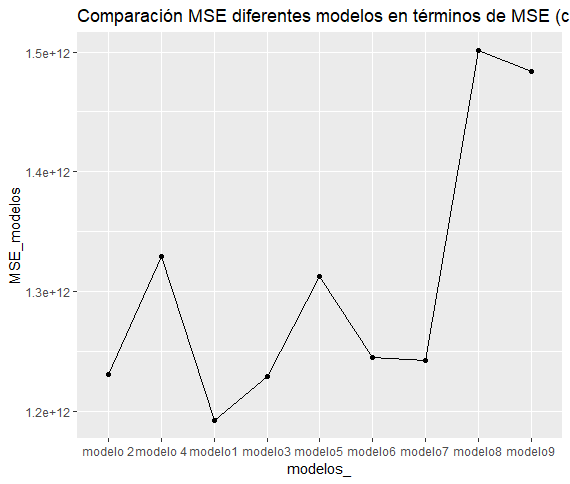
\includegraphics[width=0.4\textwidth]{../Vistas/MSE_base_training.png}}
\caption{Comparación MSE diferentes modelos base train personas}
\label{fig1}
\end{figure}

De dicha comparación, se obtiene que el modelo OLS (modelo 1) es el de menor MSE, por lo cual, es el que se escoge para realizar la regresión del Ingreso total por persona. No se reescaló el Ingreso (por ejemplo, con logaritmo), debido a que se busca obtener el valor y no una interpretación de este.\\
Luego de obtener la regresión del ingreso con los modelos presentados anteriormente, se totalizaron los ingresos por cada miembro del hogar y realizó la comparación con la línea de pobreza, es decir, se empleó la expresión presentada a continuación.  

\begin{align}
Hogar_{pobre}&=1 \textnormal{ si } Ingtot_{hogar}<Lp*Npersug\\
       &=0 \textnormal{ en caso contrario}
\end{align}
Así mismo, se realizó la comparación por Falsos negativos (obteniendo la ``Confussion Matrix'' para cada modelo con los datos del training), obteniendo igualmente que la mejor predicción se obtiene con el modelo con todas las variables consideradas.\\

Finalmente, la tabla de falsos positivos y negativos para el mejor modelo se presenta en el Cuadro ~\ref{tab_2}, en donde para la predicción en el training se obtuvo un $Accuracy=82,86\%$, y $Sensitivity=47,7\%$ para el mejor modelo.

\begin{table}[htbp]
\caption{Resumen parámetros modelo regresión}
\begin{center}
\begin{tabular}{|c|c|c|c|}
\hline
\textbf{Modelo} & \textbf{\textit{Accuracy}}& \textbf{\textit{Sensitivity}} & \textbf{\textit{False-Negatives}}\\
\hline
Modelo 1& 0,8286&0,477&17244\\
\hline
Modelo 2& 0,8294&0,272&24030\\
\hline
Modelo 3& 0,8284&0,2945&23293\\
\hline
Modelo 4& 0,799&0&33024\\
\hline
Modelo 5& 0,8119&0,23504&25262\\
\hline
Modelo 6& 0,8256&0,2187&25803\\
\hline
Modelo 7& 0,8254&0,24&25071\\
\hline
Modelo 8& 0,799&0,011&32633\\
\hline
Modelo 9& 0,8007&0,031&31997\\
\hline
\end{tabular}
\label{tab_2}
\end{center}
\end{table}


Para este modelo de regresión, el mejor modelo no fue obtenido por ningún hiperparámetro ni por ningún método de regularización, se escogió el de menor MSE, también porque en pruebas aleatorias, el parámetro Sensitivity fue mayor para este modelo OLS que para los obenidos por regularización. El modelo final fue de 6 variables, de las cuales únicamente 1 era continua (para el caso de \textit{Edad}) mientras que las otras 5 son variables categóricas, con varios niveles en el caso de la varibale \textit{Dominio}. \\
Finalmente, se procedió a realizar la predicción de los hogares pobres desde la base de datos Test hogares completa, mostrando en el Cuadro ~\ref{tab_21} el número de hogares pobres y no pobres:

\begin{table}[htbp]
\caption{Tabla de predicción}
\begin{center}
\begin{tabular}{|c|c|}
\hline
\textbf{\textit{No Pobres}}& \textbf{\textit{Pobres}}\\
\hline
54621&11547\\
\hline

\end{tabular}
\label{tab_21}
\end{center}
\end{table}





\section{Conclusiones y recomendaciones}

Se presenta en el Cuadro ~\ref{tab_20} el resumen de predicción para la base test del problem set 2. Se observa que las predicciones variarion significativamente,

\begin{table}[htbp]
\caption{Tabla de predicción resumen}
\begin{center}
\begin{tabular}{|c|c|c|}
\hline
\textbf{\textit{Approach}}&\textbf{\textit{No Pobres}}& \textbf{\textit{Pobres}}\\
\hline
Clasificación&2421&63747\\
\hline
Regresión&54621&11547\\
\hline
\end{tabular}
\label{tab_20}
\end{center}
\end{table}

De lo cual se tienen las siguientes conclusiones:

\begin{itemize}
\item Se encontró que para los modelos tanto en clasificación como en regresión, la variable \textit{Dominio} fue significativa para la predicción.
\item Se encontraron diferencias significativas en cuanto a la predicción por clasificación y por regresión a través del ingreso. Los parámetros utilizados para realizar la clasificación de Pobre o No Pobre, puede incidir.
\item La regresión del Ingreso presentó un MSE alto para todos los modelos, motivo por el cual, se puede estar dando este resultado en donde hay pobres clasificados como no pobres.
\item Los resultados más aceptables para el ejercicio, tanto de clasificación como de regresión, fueron los que tuvieron en cuenta mayor cantidad de variables que pudiesen explicar las variables dependientes en cada caso.
\end{itemize}


\end{document}
